\section{Metod}
\label{sec:joel_o-method}
För att svara på frågeställningarna har information från flera källor inhämtats. En undersökning av olika Javascript-projekt har gett kvantitativa data om deras beroenden. Denna har kompletterats med information från tidigare forskning och erfarenheter från det utförda projektet för att ge en helhetsbild över beroendens påverkan på mjukvara.

\subsection{Analys av Javascript-projekt}
\label{subsec:joel_o-method-analys}
I denna analys har beroenden för över 6~000 open-source projekt från GitHub undersökts. Ett script skrivet i Python 3 har använts för att hämta och hantera data. För lagring av data lokalt har en SQLite-databas använts. Detta är en lättviktig relationsdatabas som enkelt kan ändras från Python-scriptet. Scriptet som har använts, loggar från körningar och den slutgiltiga databasen finns tillgängliga på GitHub\footnote{https://github.com/joelnir/dependency-analysis}.

I databasen skapades tabeller för att spara data om Javascript-projekt, npm-paket och relationer mellan dem. Tabeller för intressant statistik så som hur många versionsreferenser som var ogiltiga skapades också. Ett diagram över databasen visas i figur \ref{fig:dependency-db}.

\begin{figure}[ht]
  \centering
  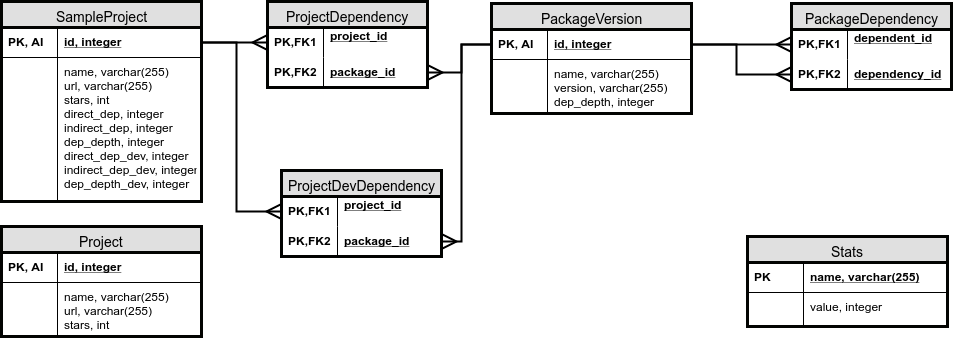
\includegraphics[scale=0.42]{npm_db}
  \caption{Databasen som har använts under undersökningen}
  \label{fig:dependency-db}
\end{figure}

Tabellerna innehåller följande:

\begin{labeling}{\textbf{ProjectDevDependency}}
  \item [\textbf{Project}] Samtliga projekt som övervägs för undersökningen
  \item [\textbf{SampleProject}] Det urval av projekt som undersöks
  \item [\textbf{ProjectDependency}] Beroenden från ett projekt till ett npm-paket i kategorin \textit{dependencies}
  \item [\textbf{ProjectDevDependency}] Beroenden från ett projekt till ett npm-paket i kategorin \textit{devDependencies}
  \item [\textbf{PackageVersion}] Specifika versioner av npm-paket
  \item [\textbf{PackageDependency}] Beroenden från ett paket till ett annat
  \item [\textbf{Stats}] Statistik om hur många beroenden som refererar till paket utanför npm-ekosystemet
\end{labeling}

Då analysen enligt frågeställning \ref{joel_o-fs:1} ska utföras på populära Javascript-projekt behövde popularitet först definieras. GitHubs system med stjärnor valdes som ett bra mått för detta. Projekt med mer än 500 stjärnmarkeringar definierades som populära. Denna gräns är godtycklig, men ger en stor datamängd att utgå ifrån.

Python-scriptet hämtade och lagrade information om dessa Javascript-projekt. En slumpmässig delmängd av dessa valdes därefter ut att ingå i undersökningen. För varje av dessa projekt utfördes sedan en analys av de beroenden som hittats i \texttt{package.json}. Antalet direkta beroenden lästes ut direkt ur \texttt{package.json}. För att undersöka indirekta beroenden användes en rekursiv metod som såg till npm-paketens vidare beroenden. Dessa undersöktes med hjälp av npm-kommandon på formen

\begin{center}
  \texttt{npm view \textit{paket}@\textit{version} dependencies \hyphen\hyphen json}.
\end{center}

Scriptet undersökte även det maximala djupet på dessa kedjor av paketberoenden från projekten. Då det även är av intresse att se hur beroenden påverkar utveckling skrevs scriptet så att det både undersöker \textit{dependencies} och \textit{devDependencies}. För en mer detaljerade beskrivning av programflödet se algoritm \ref{alg:analys} i bilaga \ref{app:algorithm}.

Då det till en början var okänt hur lång tid scriptet skulle behöva för att utföra undersökningen utfördes flera körningar med olika många utvalda projekt. Först valdes 1000 slumpmässiga paket som hade klassats som populära att ingå i undersökningen. Då scriptet kunde köras igenom under rimlig tid utfördes därefter en undersökning på samtliga projekt matchande popularitetskriteriet.

\subsection{Informationsinsamling}
För att få en mer robust förståelse för beroendens roll i Javascript utfördes en informationsinsamling av tidigare arbeten på området. Denna undersökning fokuserades på mer akademiska källor. Sökningar efter relevanta rapporter gjordes genom Google Scholar\footnote{https://scholar.google.se/} och Linköpings Universitetsbibliotek\footnote{https://www.bibl.liu.se/}.

Sökord som användes var bland annat ``Javascript'', ``npm'', ``dependencies'' och ``package''. Det var tydligt att ämnet för undersökningen var aktuellt då många av de arbeten som hittades var skrivna nyligen. Flera bra informationskällor hittades genom dessa sökningar. I dessa arbeten refererades även till andra relevanta källor som togs med i denna informationsinsamling.

\subsection{Projekterfarenheter}
I det utförda projektet har Javascript varit det huvudsakliga programmeringsspråket och npm har också använts för pakethantering. Det fanns redan i projektets kravspecifikation att vissa färdiga paket skulle användas. Detta inkluderade både stora ramverk som React och utvecklingsverktyg som ESLint.

Förutom en mängd beroenden som till en början krävdes för att påbörja arbetet tillkom flera under projektets gång. Detta inkluderade både \textit{dependencies} och \textit{devDependencies} i \texttt{package.json}. Under projektet uppkom flera öppna diskussioner om huruvida egna mjukvarukomponenter skulle implementeras eller färdiga paket användas. I dessa situationer övervägdes ofta kvalitet hos komponenterna samt till vilken grad de fyllde just det syfte som var nödvändigt.

Då projektet består av flera separata applikationer finns i slutprodukten 3 separata kodbaser med varsin \texttt{package.json}-fil. Eftersom dessa filer har befunnit sig under versionshantering under hela projektet erbjuder de en logg över hur projektets beroenden har förändrats. Dessa ändringar tillsammans med de diskussioner och konsekvenser som har omgärdat dessa har givit upphov till en mängd erfarenheter för hur beroenden påverkat projektets utveckling och till viss del även slutproduktens kvalitet.
